\documentclass[11pt]{article}

%Format and referencing 
\usepackage[letterpaper,top=2cm,bottom=2cm,left=2cm,right=2cm,marginparwidth=1.75cm]{geometry} % for setting margins VERY IMPORTANT!
\usepackage{hyperref}  % for referencing equations 
\usepackage{biblatex}  % for referencing articles 
\addbibresource{Bib.bib}


%math packages 
\usepackage{mathtools}  % allows pre-scripts and other neiche math features
\usepackage{amsmath} % equation related commands 
\usepackage{amssymb} % Fancy R ,C and other set fonts using mathbb{}
\usepackage{braket}   % for Dirac notation 
\usepackage{mathrsfs}  % for the mathscr text 

% miscellaneous
\usepackage{empheq}   % for formatting custon math boxs
\usepackage{xcolor}   % allows the defining of colours 
\usepackage[most]{tcolorbox}  % custom math boxs
\usepackage[utf8]{inputenc}   % redundant since 2018? 
%(I'm not taking out in case it breaks stuff)

\usepackage{graphicx}   % alows image insertion 
\usepackage{float}  % for making images o where you want 
\usepackage{parskip} % for getting red of paragraph indent 

\usepackage{comment} %easier multi line comments 
 \usepackage{tabularx} % for formatting tables 
 \usepackage{titling} % for making Title a variable that can be used in header 
 \usepackage{environ} % for creating and modifying environments 
 \usepackage[explicit]{titlesec}
 % for making section titles variables that can be used in header 
\usepackage{fancyhdr} % for fancy headers 

% Random commands and what not 
\numberwithin{equation}{section}

\setlength{\droptitle}{3em} 

\title{Quantum Field Theory I}
\author{Thomas Brosnan}
\date{Notes taken in Professor Samson Shatashvili class, Michaelmas Term 2024}

\DeclarePairedDelimiterXPP\BigOSI[2]%
  {\mathcal{O}}{(}{)}{}%
  {\SI{#1}{#2}}

\newtcbox{\mymath}[1][]{%
    nobeforeafter, math upper, tcbox raise base,
    enhanced, colframe=blue!30!black,
    colback=blue!30, boxrule=1pt,
    #1}
\tcbset{highlight math style={boxsep=2mm,,colback=blue!0!green!0!red!0!}}

\newenvironment{bux}{\empheq[box=\tcbhighmath]{align}}{\endempheq}
\newenvironment{bux*}{\empheq[box=\tcbhighmath]{align*}}{\endempheq}
\renewenvironment{flalign}{\vspace{-3mm}\empheq[box=\tcbhighmath]{align}}{\endempheq}
\renewenvironment{flalign*}{\vspace{-3mm}\empheq[box=\tcbhighmath]{align*}}{\endempheq}
%\renewenvironment{align}{\vspace{-5mm}\begin{align}}{\end{align}}
%\renewenvironment{align*}{\vspace{-5mm}\begin{align*}}{\end{align*}}
\renewenvironment{alignat}{\empheq{align*}}{\endempheq}


\newcommand{\hsp}{\hspace{8pt}}

\newcommand*{\sectionFont}{%
  \LARGE\bfseries
}

\newenvironment{eq}{\begin{equation}}{\end{equation}}
    


\makeatletter
\let\Title\@title % Copy the title to a new command
\makeatother

%change this RGB value to change the section background colour 
\definecolor{mycolor1}{RGB}{125, 187, 242}
\colorlet{SectionColour}{mycolor1}
%subsection background colour 
\definecolor{mycolor2}{gray}{0.8}
\colorlet{subSectionColour}{mycolor2}
%subsubsection background colour 
\definecolor{mycolor3}{RGB}{255,255,255}
\colorlet{subsubSectionColour}{mycolor3}



\begin{document}

\maketitle

\newpage
\topskip0pt
\vspace*{\fill}
\begin{center}
\Large
    "If you can't explain it simply enough you don't understand it well enough"
    
    - Albert Einstein
\end{center}
\vspace*{\fill}
\newpage 
\tableofcontents
% For \section
 \titleformat{\section}[block]{\sectionFont}{}{0pt}{%
 \fcolorbox{black}{SectionColour}{\noindent\begin{minipage}{\dimexpr\textwidth-2\fboxsep-2\fboxrule\relax}\thesection  \hsp #1 {\strut} \end{minipage}}}
% For \subsection
 \titleformat{\subsection}[block]{\bfseries}{}{0pt}{%
 \fcolorbox{black}{subSectionColour}{\noindent\begin{minipage}{\dimexpr\textwidth-2\fboxsep-2\fboxrule\relax}\thesubsection  \hsp #1 {\strut} \end{minipage}}}
% For \section*
 \titleformat{name=\section, numberless}[block]{\sectionFont}{}{0pt}{%
 \fcolorbox{black}{SectionColour}{\noindent\begin{minipage}{\dimexpr\textwidth-2\fboxsep-2\fboxrule\relax} #1 {\strut} \end{minipage}}}
  % For \subsection*
 \titleformat{name=\subsection, numberless}[block]{\bfseries}{}{0pt}{%
 \fcolorbox{black}{subSectionColour}{\noindent\begin{minipage}{\dimexpr\textwidth-2\fboxsep-2\fboxrule\relax} #1 {\strut} \end{minipage}}}
 % For \subsubsection
 \titleformat{\subsubsection}[block]{\bfseries}{}{0pt}{%
 \fcolorbox{black}{subsubSectionColour}{\noindent\begin{minipage}{15cm}\thesubsubsection \hsp #1 {\strut} \end{minipage}}}
  % For \subsubsection*
 \titleformat{name=\subsubsection, numberless}[block]{\bfseries}{}{0pt}{%
 \fcolorbox{black}{subsubSectionColour}{\noindent\begin{minipage}{15cm} #1 {\strut} \end{minipage}}}
\newpage 
%header 
\pagestyle{fancy}
\fancyhf{} % Clear all header and footer fields
\fancyhead[L]{\Title}
\fancyhead[R]{\nouppercase{\leftmark}}
\fancyfoot[C]{-~\thepage~-}
\renewcommand{\headrulewidth}{1pt}





%starting document 
\normalsize
\newpage
\section{Section}

\subsection{Theorem:} let $A$ be an element of $R$ such that:
\begin{align}
\begin{split}
    c_i = \langle\psi|\phi\rangle ,~~~~ c_i = \langle\psi|\phi\rangle  \\
    c_i = \langle\psi|\phi\rangle ,~~~~ c_i = \langle\psi|\phi\rangle
\end{split}
\end{align}

%the bux 

Then the final result is:

\begin{bux}
\begin{split}
    c_i = \langle\psi|\phi\rangle ,~~~~ c_i = \langle\psi|\phi\rangle  \\
    c_i = \langle\psi|\phi\rangle ,~~~~ c_i = \langle\psi|\phi\rangle
\end{split}
\end{bux}

\begin{figure}
\centering
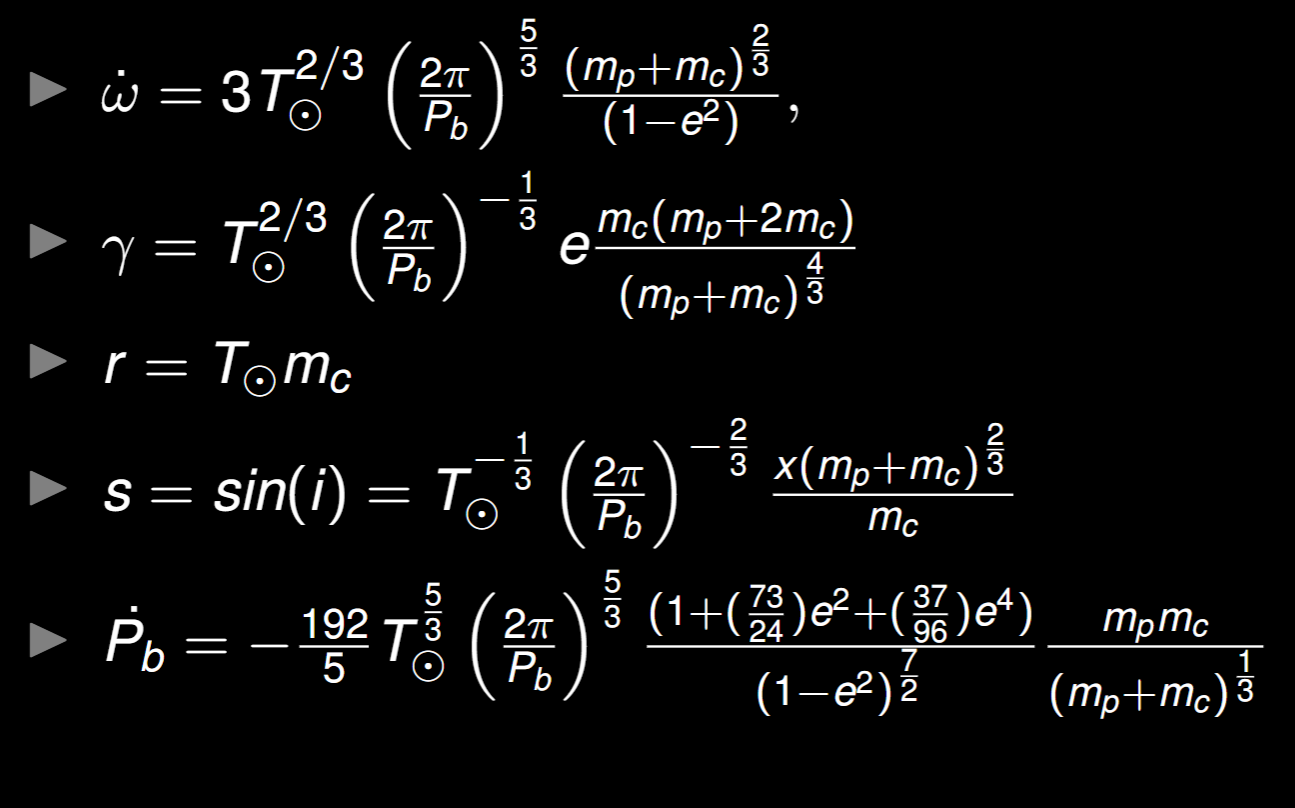
\includegraphics[width=0.8\textwidth]{Screenshot 2023-06-15 172321.png}
\caption{\label{fig:2}\emph{Diagram of the experimental setup circuit}}
\end{figure}

\newpage
let $A$ be an element of  such that:

\begin{align}
\frac{1}{2} =  1/2 +0 -0
\end{align}

\end{document}
